%%%%%%%%%%%%%%%%%%%%%%%%%%%%%%%%%%%%%%%%%%%%%%%%%%%%%%%%%%%%
%% Capítulo 5 / Resultados
%%%%%%%%%%%%%%%%%%%%%%%%%%%%%%%%%%%%%%%%%%%%%%%%%%%%%%%%%%%%
\chapter{Resultados}
\epigrafe{Everyone in this country should learn how to program a computer, because it teaches you how to think.}
              {\textsc{Steve Jobs}}

\section{Ejemplo Tabla}
\lipsum[1].  
Los resultados pueden verse en la Tabla \ref{tab:Tabla1}

\begin{table}[htbp]
\centering
\caption{Resultados obtenidos.}
\label{tab:pversust}
\begin{tabular}{ccc}
\toprule
\textbf{Parametro A } & \textbf{Resultado } \\
\midrule
A & 1 \\
B & 2 \\ 
C & 3 \\
D & 4 \\
\bottomrule
\end{tabular}
\label{tab:Tabla1}
\end{table}

\lipsum[2]

\section{Ejemplo Figura}
\lipsum[3-4]

\begin{figure}[htbp]
\centering
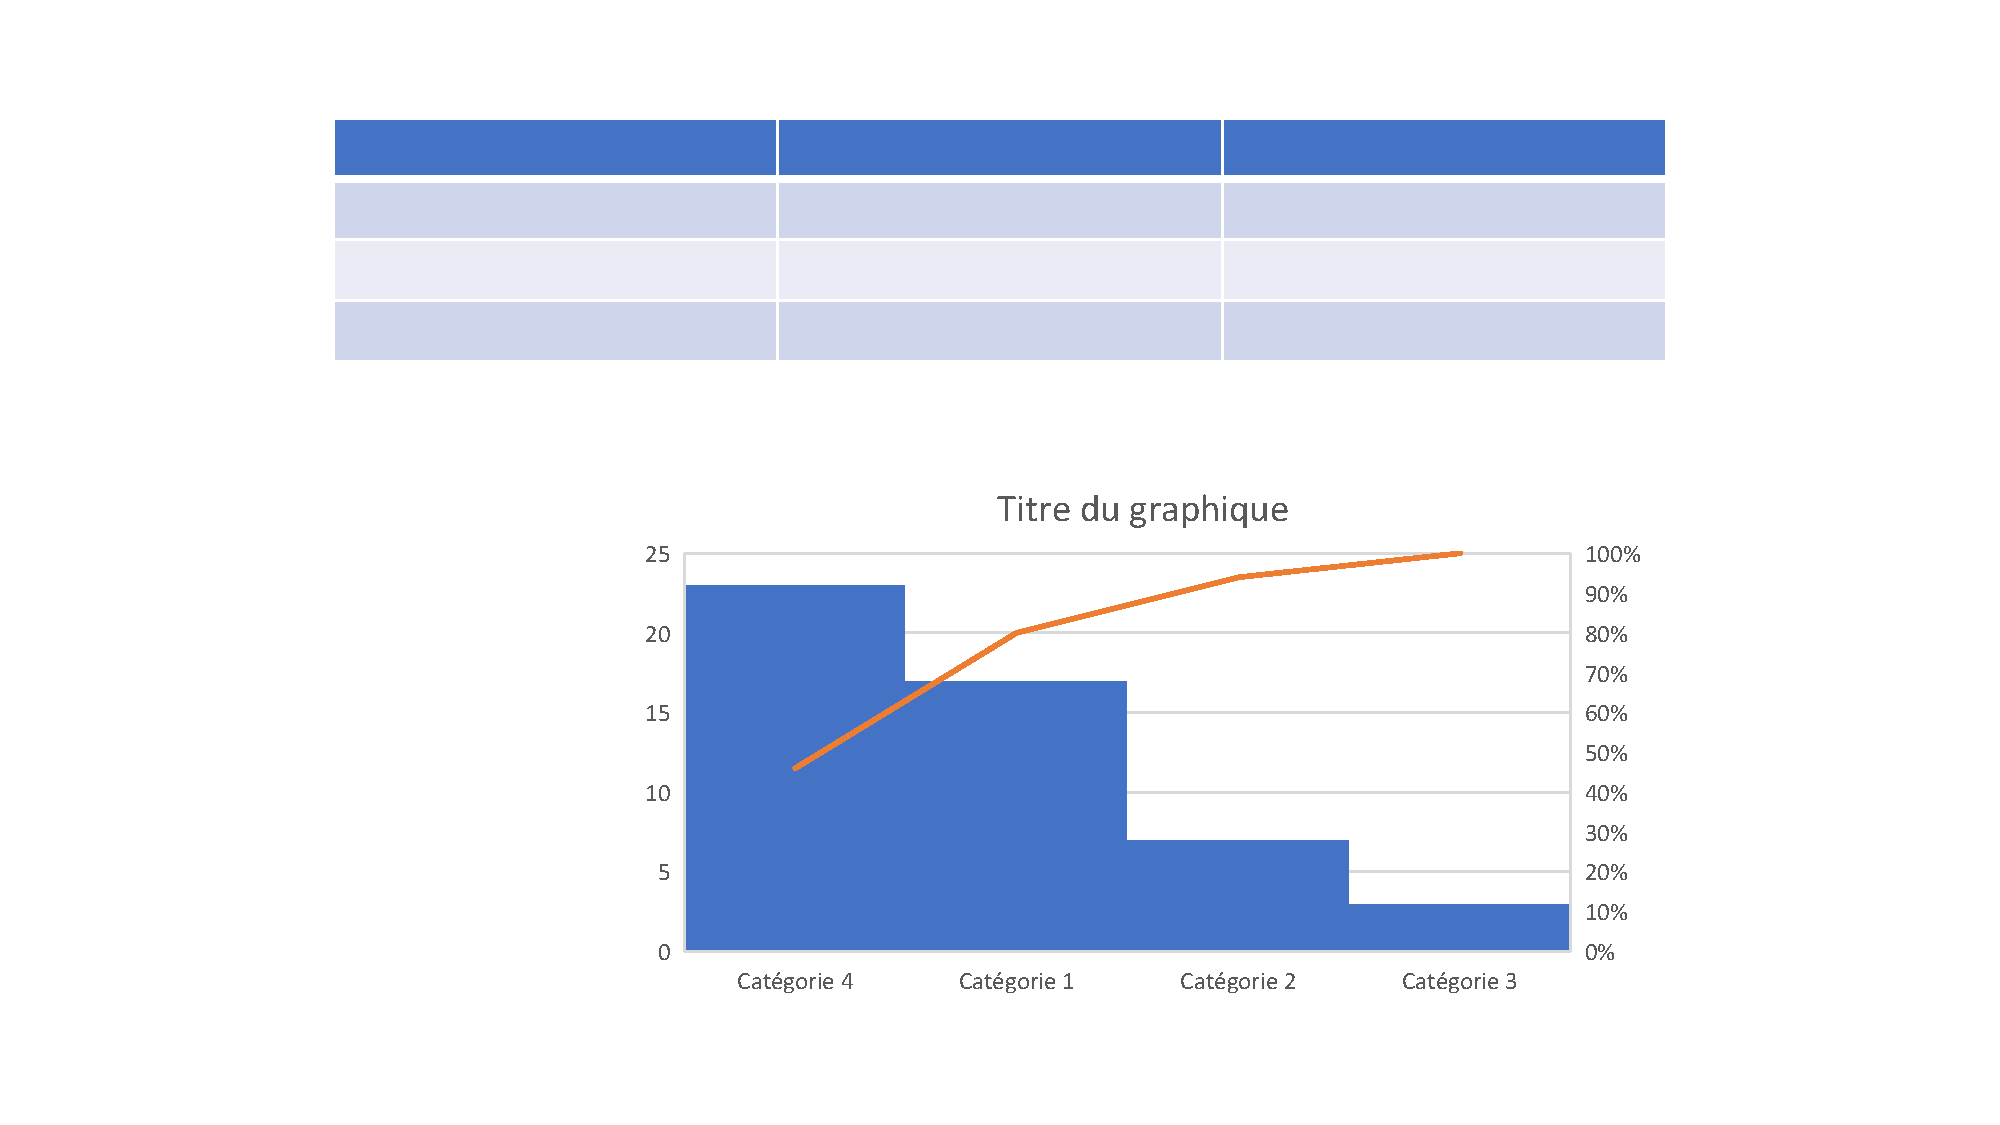
\includegraphics[width=0.50\textwidth]{e_Imagen01}
\caption{Duis eget orci sit amet orci dignissim rutrum.}
\label{fig:particion}
\end{figure}

\section{Tercera sección}
\lipsum[5-6]
